%%%%%%%%%
%
% The International Trade Network Origins of Domestic Fluctuations
% Research notes
% Brian Dew
%
%%%%%%%%%
	\documentclass[10pt,letterpaper,pdftex]{article}

%
% Packages
%
	\usepackage[pdftex]{graphicx}	
	\usepackage[right=1.6in, left=1.6in, top=1.6in, bottom=1.6in]{geometry}
	\usepackage{pgfplots,pgfplotstable}
	\usepackage{amsmath,amsthm,amssymb}	
	\usepackage[colorlinks,
  		linkcolor=cyan!30!blue!80!black,
  		filecolor=cyan!30!blue!80!black,
 		citecolor=cyan!30!blue!80!black,
 		urlcolor=cyan!30!blue!80!black,]{hyperref}
	\usepackage{calc}
	\usepackage[latin1]{inputenc}
	\usepackage{float}
	\usepackage{array}
	\usepackage{booktabs}
	\usepackage[]{caption}
	\usepackage{xcolor}
	\usepackage[eulergreek]{sansmath}
	\usepackage{listings}
	\usepackage{parskip}
	\usepackage{bm}
	\usepackage{subcaption}
	\usepackage{soul}
	\usepackage{fancyhdr}
	\usepackage[nottoc,numbib]{tocbibind}
	\usetikzlibrary{automata, arrows}
	\usepackage[activate={true,nocompatibility},final=true,kerning=true,
		spacing=true,tracking=true,shrink=30,stretch=30,factor=0]{microtype}
		
\usepackage{sectsty}
\sectionfont{\usefont{T1}{qhv}{b}{n}\selectfont\Large} 
\subsectionfont{\usefont{T1}{qhv}{b}{n}\selectfont\large} 
\subsubsectionfont{\usefont{T1}{qhv}{b}{n}\selectfont\normalsize} 
 
\pagestyle{fancy}
\fancyhf{}
\rhead{}
\lhead{\leftmark}
\cfoot{\thepage}

\pgfplotsset{compat=newest}

\newcommand{\invisiblesection}[1]{%
  \phantomsection%
  \stepcounter{section}%
  \addcontentsline{toc}{section}{\protect\numberline{\thesection}#1}%
  }


%
% Title Info
%

	\author{Brian W. Dew\thanks{This paper benefits from constructive feedback from Professor Kara Reynolds and Professor Amin Mohseni-Cheraghlou, both American University Department of Economics. The research builds on work with Yevgeniya Korniyenko and Magali Pinat, both International Monetary Fund. Results were produced using Stata and Python's networkX and powerlaw packages, see: \url{https://github.com/bdecon/trade_network}. All errors in this paper are my own.}\\ (brian.dew@american.edu)}
	\title{The International Trade Network Origins of Domestic Fluctuations}

\tikzset{
    	every node/.append style={font=\sansmath\sffamily\footnotesize}}

\begin{document}
\maketitle
\begin{abstract}
    Recent empirical and theoretical work identifies network structure as a determinant of which microeconomic shocks cause aggregate output fluctuations. Evidence suggests international trade networks have the same role in determining how localized supply shocks transmit across borders and whether they propagate. Two models are applied to international trade data to identify the relationship between the international trade network structure for individual goods, countries' role in trade networks, and exogenous shocks to supply and demand. Countries which import goods that have power-law distributed exporter shares are shown to face output fluctuations, particularly in response to supply shocks in the network. Recent developments in trade network structure, particularly for the trade of oil and gas, are discussed.
\end{abstract}

\newpage

\tableofcontents

\newpage

\section{Introduction} \label{intro}

Economists have long discussed how (and whether) idiosyncratic shocks affect the larger economy (Lucas 1977, Kydland and Prescott 1982, Jovanovic 1987). Recent research examines how networks, the relationship between economic agents, provide a linkage between idiosyncratic shocks and macroeconomic outcomes (Gabaix 2011, Carvalho 2008, Acemoglu et al 2012, Chaney 2014).  Within this discussion, one area that has received less focus, but provides useful insight, is the international trade network effects of localized supply shocks, such as those caused by natural disasters. 

In the context of renewed discussion on trade and globalization, and the search for a better understanding of the interconnections between agents, network analysis offers a valuable set of tools and a unique vantage point for studying international trade. Trade liberalization and the rise of global value chains has dramatically changed the techniques and locations of the production of goods. The often large number of connections between firms producing goods, their upstream suppliers, and their downstream customers, are well represented as a network, which permits simultaneous examination of the full set of relationships rather than individual bilateral interactions. Networks provide a simple and powerful framework for determining how activity and outcomes are distributed within a complex system, and how the system responds to shocks. 

This paper examines the intersection of these three relevant topics: \textsl{shocks} that affect individual agents, \textsl{connections} between agents, and the \textsl{distribution} of activity. Specifically, two models are applied to international trade data to explain relationships between exogenous shocks and fluctuations elsewhere in the network. The paper makes an attempt to answer the question: how does the distribution of suppliers and the connections between economic agents determine whether idiosyncratic shocks die out or propagate?

The first model examines aggregate fluctuations at a country level by decomposing each country's imports of individual intermediate goods by whether or not each good has power-law-distributed exporter sizes, and whether or not the good is imported from a country with a large natural disaster. Imports of goods that have few central suppliers from countries with a natural disaster supply shock are expected to negatively affect aggregate output in the next period, as measured by a country's exports. That is, intermediate good flows are affected by the negative supply shock, and the consequences of this depend in part on whether alternative suppliers are available. 

The second model examines instead exogenous shocks that are not localized, but captured by the price of oil and its interaction with each country's role in the global trade network of all goods. Intuitively, countries tightly interwoven into global supply chains, for example, are expected to see larger aggregate fluctuations from exogenous changes to supply and demand. Network analysis provides tools to measure the role of each country within the global trade network, which is assessed over time.

Additionally, to better explain the models and demonstrate the usefulness of their results, the international trade of oil and gas is examined in detail in this paper. Oil and gas combine to claim nearly 15 percent of the international trade of goods, and are used as inputs to all sectors and nearly all firms, either through production or transportation costs. Network analysis is used to show how the role of oil and gas within international trade has evolved and how the role of individual countries in the global trade network for energy has also shifted. 

The paper proceeds as follows: section 2 offers a review of the literature on network analysis and trade, section 3 describes the economic theory behind the research, section 4 serves as the core of the paper and explains both models, including the network analysis measures used and the data sources, section 5 presents the results of econometric tests of the models, and section 6 offers the conclusion and describes areas for additional study.


\section{Literature Review} \label{litrev}

Networks have long been a natural way to represent related sets of bilateral relationships, including social connections between people in a group, connections between suppliers and producers in an economy, and the global trade of goods and services between countries. Early examinations of international trade as a network include Snyder and Kick (1979), Nemeth and Smith (1985), and Smith and White (1992). A recent and thorough description of the world trade network comes from De Benedictis and Tajoli (2011) who provide a detailed description of network analysis tools and note the presence of changes in network structure over time. Countries have as a whole become more interconnected, but also more heterogeneous in their role in networks (IMF 2011). 

Rather than describing the trade network, economists are more often interested in using network analysis to explain real world phenomena. Glick and Rose (1999) found evidence that currency crises spread through trade channels more than they can be explained within a country by macroeconomic or financial fundamentals. Likewise, network analysis has been used to study financial contagion from interconnections in the banking sector and how this poses systemic risk (Minoiu and Reyes 2011). This work examines how otherwise localized shocks spread through international trade networks.

Meanwhile microeconomic foundations emerge and connect network structures, empirical observations, and economic theory. In 2011, Xavier Gabaix shows, counter to the argument of Lucas (1977) that idiosyncratic shocks average out and have no aggregate impact, the idiosyncratic movements of the largest 100 U.S. firms explain about one-third of aggregate output fluctuations. The fat-tailed distribution of firm sizes results in idiosyncratic shocks that do not die out, which suggests that macroeconomic questions can be partially answered by looking at large firms. Gabaix notes the potential extension of this theoretical concept to international trade. 

Critically, Acemoglu et al (2012) identify the network of input-output (I-O) linkages between sectors as the mechanism through which idiosyncratic shocks spread and can lead to aggregate fluctuation. Through the I-O network, idiosyncratic shocks can have cascade effects on downstream customers and thereby the entire economy. When one firm supplies many other firms in the economy shocks propagate. This work identifies products with relatively few, but important, suppliers.

Work has been done on trade network structure and growth, such as Kali, Mendez \& Reyes (2007), where increasing the number of trading partners by 10 is shown to increase growth by 0.52 percentage points. Additionally, Duenas and Fagiolo find that imbalances in international trade are are not satisfactorily explained by a gravity model, but are found to have a similar topology to the international trade network. This paper looks at low-frequency and low-probability but high impact situations (such as severe shocks) as a tool for explaining an additional portion of fluctuations to economic aggregates.

The other vein of network analysis research in trade is related to how shocks propagate, which can borrow from the microfoundations identified by Gabaix and Acemoglu et al. One such example is by Contreras and Fagiolo (2014), who use diffusion models examine how shocks propagate through the I-O network in EU countries. Authors determine the impact of a shock to largely depend on the type of shock and size of the country, with large countries being the most vulnerable. My research offers a similar technique and conceptual framework but analyzes international trade networks, and focuses specifically on natural disasters and shocks to the price of oil.

Recent work on network analysis of trade has extended to examinations of individual products. In the energy sector, this includes papers on the features and evolution of crude oil. An et al (2014) note that the size of the network for crude oil increased between 1993 and 2012, but the number of connections between countries increased more rapidly than the number of exporting countries. The network has become more stable and interconnected over time. Geng et al (2014) analyze the trade network for natural gas, which is quite different from that of crude oil. There is a distinct lack of integration between the trade networks in North America, Asia, and Europe, driven in part by differences in LNG access and pipeline connections, and by political factors.  

Unlike the previous research, this work examines the differences between the trade network structures of various goods at a dis-aggregated level of specificity. Further, I examine what implication this has for the transmission of shocks, and how the transmission of shocks can thereby affect aggregate outcomes. Additional consideration is given to the distribution of features within a network, and the dynamic aspects of shock propagation.


\section{Model} \label{models}
\subsection{Theoretical background} \label{modelstheory}
Xavier Gabaix (2011) offered theoretical and empirical evidence against the argument of Lucas (1977) that firm-specific shocks average out. Gabaix showed that 1/3 of output volatility in the United States can be directly tied to changes in the 100 largest U.S. firms. When firm sizes follow a power-law distribution, idiosyncratic shocks do not average out, and actually propagate downstream and affect aggregate economic output. This is because there are often few central suppliers for the key inputs to several industries. A shock to one the central firms causes consequences for all firms that require the input for their own production. I hypothesize that this relationship holds internationally, particularly given actual variation in the volume of exports by product and country, and the rise of international trade of intermediate goods due to global value chains. 

In addition to evidence at a firm and national level, anecdotal evidence suggests the existence of an international counterpart to the domestic observation of Gabaix. For example, motivation for this research comes from an anomaly noticed following two recent natural disasters. First, the 2011 Tohoku earthquake and tsunami, which caused massive destruction, loss of life, and a nuclear disaster, also caused supply-shocks in global trade. Automotive assembly lines around the world were forced stop production after key intermediate inputs from Japan were delayed (Canis 2011, Carvalho 2014). Likewise, the launch of the iPad 2 was delayed when the Japanese supplier of the cover glass was affected by the disaster (Lohr 2011). Second, the 2011 Thailand floods disrupted the production of computer hard disk drives, which has been dominated by Thai producers (Fuller 20ll). The price of hard disk drives nearly doubled worldwide and remained elevated for two years, following the disruption caused by the floods (Hruska 2013). Such disruptions to the supply of key intermediate goods can create a situation where a localized supply-shock (from a natural disaster) results in aggregate fluctuations elsewhere in the world.

Essentially, if localized shocks are large enough, and production processes subject to power-law distributed suppliers, alternative international and domestic suppliers will not be able to absorb shocks to production by increasing their own output. In these cases, the absence or delay of a crucial intermediate good causes the delay or reduction of domestic value added. A visual example offers additional support for the fundamental argument that upstream shocks, dependent upon the availability of alternative suppliers, determine downstream outcomes (figure 1). 


\subsubsection*{\centerline{Visual representation: shock to central vs. non-central supplier}}
\vspace{1mm}
\begin{figure}[ht]
\caption[]{The effect of a negative shock to Australian iron ore exports depends on network structure. Here circles represent countries, with Australia (AUS) as the localized supply-shock affected country, in red, countries without a functioning supplier in orange, and unaffected countries in blue\footnotemark. Solid lines represent unaffected trade flows and dashed lines represent compromised trade flows.} \label{fig:M1}
\centering
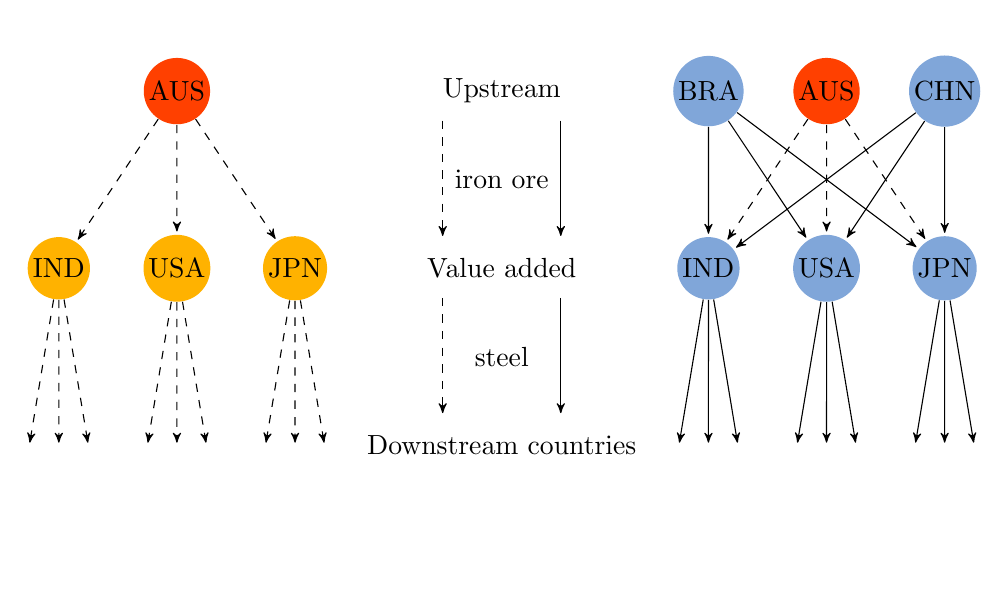
\begin{tikzpicture}
  [>=stealth',shorten >=1pt,scale=0.75, 
  	auto=left,every node/.style={inner sep=1pt,circle,fill=orange!60!yellow
  		}
  ]
  \node [fill=red!50!orange] (n6) at (3,10) {AUS};
  \node [draw=none,fill=none] (n7) at (8.5,10) {Upstream};
  \node [draw=none,fill=none] (n8) at (8.5,7) {Value added};
  \node [draw=none,fill=none] (n9) at (8.5,8.5) {iron ore};
  \node [draw=none,fill=none] (n10) at (8.5,4) {Downstream countries};
  \node [draw=none,fill=none] (n11) at (8.5,5.5) {steel};
  \node (n4) at (5,7)  {JPN};
  \node (n5) at (1,7)  {IND};
  \node (n3) at (3,7)  {USA};
  \draw [->, dashed] (7.5,9.5) -- (7.5,7.5);
  \draw [->] (9.5,9.5) -- (9.5,7.5);
  \draw [->, dashed] (7.5,6.5) -- (7.5,4.5);
  \draw [->] (9.5,6.5) -- (9.5,4.5);
  \draw [->, dashed] (n4) -- (5,4);
  \draw [->, dashed] (n4) -- (4.5,4);
  \draw [->, dashed] (n4) -- (5.5,4);
  \draw [->, dashed] (n5) -- (1,4);
  \draw [->, dashed] (n5) -- (0.5,4);
  \draw [->, dashed] (n5) -- (1.5,4);
  \draw [->, dashed] (n3) -- (3,4);
  \draw [->, dashed] (n3) -- (2.5,4);
  \draw [->, dashed] (n3) -- (3.5,4);
  
  \foreach \from/\to in {n6/n4,n6/n5,n6/n3}
    \draw[->, dashed] (\from) -- (\to);
    
  \node [fill=red!50!orange] (p6) at (14,10) {AUS};
  \node [fill=blue!70!green!50] (p2) at (12,10) {BRA};
  \node [fill=blue!70!green!50] (p1) at (16,10) {CHN};  
  \node [fill=blue!70!green!50] (p4) at (16,7)  {JPN};
  \node [fill=blue!70!green!50] (p5) at (12,7)  {IND};
  \node [fill=blue!70!green!50] (p3) at (14,7)  {USA};
  \draw [->] (p4) -- (16,4);
  \draw [->] (p4) -- (15.5,4);
  \draw [->] (p4) -- (16.5,4);
  \draw [->] (p5) -- (12,4);
  \draw [->] (p5) -- (11.5,4);
  \draw [->] (p5) -- (12.5,4);
  \draw [->] (p3) -- (14,4);
  \draw [->] (p3) -- (13.5,4);
  \draw [->] (p3) -- (14.5,4);

  \foreach \from/\to in {p2/p3,p2/p4,p2/p5,p1/p5,p1/p3,p1/p4}
    \draw[->] (\from) -- (\to);
    
  \foreach \from/\to in {p6/p4,p6/p5,p6/p3}
 	\draw[->, dashed] (\from) -- (\to);
\end{tikzpicture}
\end{figure}
\footnotetext{There may still be price effects.}

Therefore, there are three basic elements to my argument: the connections between countries, the distribution of suppliers, and the existence of exogenous shocks. First, countries need goods to produce goods; the inputs from upstream suppliers are required to produce outputs for downstream customers. In economics, this process is usually described as the Leontief input-output linkages between sectors or firms in the economy. Given the rise of global value chains and other changes to the structure of production, many times these linkages cross borders.

Next, countries role in the trade of individual goods, and in the global trade network in general, is not uniform. Specifically, the exporter shares of certain goods follows a power law distribution\footnote{Defined for this paper as having an estimated alpha value of weighted out-degree centrality scores between 2 and 3, where $p(x) = Cx^{-\alpha}$.}. The extent of this distribution varies from product to product, and can be captured for each product by applying the tools of network analysis. Additionally, some countries are more influential in the global trade network, not only because of what they produce, but also because of which countries they supply.

Third, shocks from upstream are propagated downstream depending on the network structure for the affected product. These shocks can be idiosyncratic or general, but are assumed to be exogenous to each country that is not directly affected by a localized idiosyncratic shock. Such impulses to a network provide the mechanism through which the effects of network structure can be studied.

\subsection{Microfoundation} \label{modelsmicro}

The derivation from economic theory of a testable hypothesis is borrowed almost verbatim from Acemoglu, Akcigit, and Kerr (2016) but adjusted to apply internationally (and to ignore demand shocks) as follows:

First, define a Cobb-Douglas production function for each country:

\begin{equation*}
y_i = e^{z_i}l_i^{\alpha_i^l} \prod_{j=1}^{n} x_{ij}^{a_{ij}},
\end{equation*}

where $x_{ij}$ is the volume of goods produced by country j and imported to country i, $l_i$ is labor, and $z_i$ is a Hicks-neutral productivity shock. Assume that for each country, $\alpha_i^l >0$, and $a_{ij} \geq 0$ for each pair of countries in the network (if $a_{ij} = 0$, there are no imports to country $i$ from country $j$). Lastly,

\begin{equation*}
 \alpha_i^l + \sum_{j=1}^{n} a_{ij} = 1
\end{equation*}

so constant returns to scale are assumed. 

The market clearing condition is:
\begin{equation*}
y_i = c_i + \sum_{j=1}^{n} x_{ji}
\end{equation*}

where $c_i$ is domestic consumption and an amount of goods is also exported to each of $n$ countries.

The downward sloping line comes from preferences of a representative household:
\begin{equation*}
u(c_1,c_2,...,c_n,l) = \gamma (l) \prod_{i=1}^{n} c_i^{\beta_i}
\end{equation*}

where $\beta_i$ is distributed between 0 and 1, sums to 1 across all $i$'s, and represents the weight of goods from country $i$ in the representative household's preferences. The dis-utility of labor is given by the function $\gamma (l)$, which is assumed to be negative.

The household faces the following budget constraint:
\begin{equation*}
 \sum_{i=1}^{n} p_ic_i = wl
\end{equation*}

where $w$ is the wage rate, set to 1 for simplicity.

Aggregate profit maximization applied to the Cobb-Douglas production functions determines the individual good trade flows (assuming for simplification that trading costs are CIF and incorporated into $p_j$):
$$ \frac{p_jx_{ij}}{p_iy_i} = a_{ij}$$

Consider therefore an international input-output matrix of $a_{ij}$'s denoted as \textbf{A}:
\begin{equation*}
\text{\textbf{A}} = \begin{bmatrix}
		a_{11} & a_{12} & ... \\
		a_{21} & a_{22} &  \\
		\vdots &  & \ddots 
		\end{bmatrix}
\end{equation*}		

The Leontief inverse of matrix \textbf{A} is defined as:
\begin{equation*}
 \mathbf{H} \equiv (\mathbf{I} - \mathbf{A})^{-1} 
\end{equation*}


with each entry in matrix \textbf{H} identified as $h_{ij}$.

Acemoglu, Akcigit, and Kerr then propose the following relation for the impact of domestic and foreign shocks on changes to aggregate output:
\begin{equation} \label{eq:main_aak}
 d \ \text{ln} \ y_i = \underbrace{dz_i}_{\text{own effect}} + \underbrace{\sum_{j=1}^{n} (h_{ij} - \bm{1}_{j=i}) \times dz_j}_{\text{network effect}}
\end{equation}

where $\bm{1}_{j=i}$ is the indicator function for $j=i$.

Equation \ref{eq:main_aak} explains fluctuations in aggregate output for country $i$ as the combination of domestic idiosyncratic shocks, the connections to other countries through the trade of goods, and both the existence and importance to country $i$ of shocks to other countries. Shocks to country $j$ will affect country $i$ if the existing level of trade between the countries is large and also if there are few alternative suppliers. 

\section{Methodology and Data} \label{data}
Econometric tests of the theory require estimates both of the distribution of supplier sizes and the role of each country in the global trade network, which is obtained by using the tools of network analysis. Shocks, which for the purpose of this research must be exogenous, are identified using data on natural disasters and the price of oil. This section describes the techniques used to generate estimates for econometric analysis, and discusses the mathematical, statistical, and economic support for the variable selection. 

\subsection{Network analysis: overview and centrality} \label{nw1}
Representing global trade relationships as a complex network provides insight into developments that affect individual members of the network but cannot necessarily be observed in bilateral relationships. This section first offers a brief primer on international trade represented as a network and a discussion of the network analysis concepts of centrality and degree distribution. Data sources are then discussed, followed by a presentation of two models which aim to test the relationship identified through economic theory. 

\subsubsection{Network overview} \label{nw2}
To begin the network analysis, each country involved in the international trade of a good or set of goods is identified as a `node'. Each node may either produce a good and supply it another country as an export, or consume a good produced in another country as an import. These exports and imports comprise the trade flows between countries and are represented in a network as an `edge', usually shown as a line or arrow connecting two nodes. Each edge contains important information about the flow of goods between two countries. First, each edge is `directed' as the flow of goods exits the exporter node and enters the importer node. Edges directed outward from a node represent that nodes' exports, while edges directed inward to the node represent its imports. Additionally, in the global trade network each edge contains `weights', which are the value and quantity of goods associated with the trade flow.

\begin{figure}[!htb]\label{fig:nw_simple}
  \caption{Single trade flow, exports from country $i$ to country $j$, as a `network'}
  {\centering
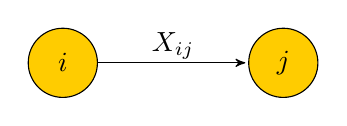
\begin{tikzpicture}[>=stealth',shorten >=1pt,auto,node distance=2.8cm,every node/.style={inner sep=1pt}]
  \node[state,fill=orange!40!yellow] (q1)      {$i$};
  \node[state,fill=orange!40!yellow]         (q2) [right of=q1]  {$j$};
  \path[->]          (q1)  edge                 node {$X_{ij}$} (q2);
\end{tikzpicture}\\}
\end{figure}

Even a simple bilateral trade flow can be represented as a network (figure 2). To build the complete network, I continue to add nodes and edges until all flows are included. Once a complete network is constructed, additional techniques for describing individual nodes, as well as the overall structure of the network, become available.

\subsubsection{Degree and eigenvector centrality} \label{nw3}
One simple measure of how an individual node is related to its network is the number of connections it has to other nodes, referred to as its `degree'. In international trade a country's degree is its total number of trading partners. As with edges, the degree of a node is directed. The out-degree of a node measures the number of nodes to which it is connected through its exports, while the in-degree of a node captures the number of nodes it is connected to through imports. That is, if country $i$ exports good $k$ to nine countries and imports good $k$ from three countries, its out-degree is nine and its in-degree is three. Degree can also be `weighted' to capture the total value of directed flows.  The weighted out-degree corresponds to the total value or quantity of exports (depending on which is used as the weight), while the the weighed in-degree is the total value of quantity of imports. 

Often researchers are interested in how a node compares with other nodes in its network. There are several ways to compare the role of individual nodes, with various measures of `centrality' being the most common. Centrality captures the influence that an individual node has in its network, and very influential nodes are colloquially referred to as `central players'. Two distinct measures of centrality are degree centrality and eigenvector centrality. 

The degree centrality of a node is the share of other nodes to which it is connected. The out-degree centrality measures the share of importers that are serviced by each exporter, while the in-degree centrality captures the share of exporters that service each importer. I represent the out-degree centrality of country $i$ in network $g$ comprised of $n$ nodes, $C_i^{\text{out}}(g)$, as its number of exporting edges (out-degree), $k_i^{\text{out}}$, divided by the total number of possible import partner nodes, $(n-1)$:
\begin{equation} 
C_i^{\text{out}}(g) = \frac{k_i^{\text{out}}}{(n-1)}
\end{equation}
The out- and in-degree centrality of a country, in international trade terms, is its export- and import- share of trade, respectively. The weighted version of out-degree, used in this paper, simply replaces the number of edges with the total value of the edges, and replaces the number of possible partners with the total value of trade in the network.

Each network indicator described in this section has a direct and simple international trade analog. However, one crucial graph theory addition to existing measures of a country's role in trade is eigenvector centrality\footnote{Google search results rely of a variation of eigenvector centrality named after Larry Page, called the PageRank algorithm. The search results are ordered based not only on the relevance of the individual webpage, but importantly on how many other pages link to the page, and how relevant those other pages are.}. Eigenvector centrality, proposed by Bonacich (1972) but pioneered by Leontief, approaches the question of influence in a network to incorporate both the role of a country in the network, but also the role (and influence) of its partners. The eigenvector centrality of country $i$ in network $g$ is proportional to the sum of the centrality of its trading partners, indexed by $j$:

\begin{equation}\label{eq:evc}
\lambda C^e_i(g) = \sum\nolimits_{j} g_{ij}C^e_j(g)
\end{equation}

where from \eqref{eq:evc} in matrix notation, $\lambda C^e(g) = gC^e(g)$, and the constant $\lambda$ is the corresponding eigenvalue for the network eigenvector $C^e(g)$. The eigenvector associated with the largest eigenvalue is the estimated centrality. This measure can incorporate both trade flow direction and weights. The import centrality is the left-hand eigenvector of the adjacency matrix $g$ associated with eigenvalue $\lambda$.

\subsection{Network analysis: degree distribution} \label{nw4}
In addition to measures which examine the role of each country, measures which cover the entire trade network provide information on the size and structure of the market. As discussed in section \ref{modelstheory}, the distribution of supplier sizes is of economic importance, particularly if it follows a power law distribution. In network analysis, the distribution of connections in a network is referred to as the degree distribution. 

The relative frequency of exporter sizes in the trade network is represented as $p(x)$, the fraction of nodes with weighted out-degree $x$ under probability distribution $p$. This paper focuses on the distribution of exporter sizes, as measured by the weighted out-degree distribution, however, the distribution of importer sizes by product has additional economic significance.

The distribution of exporter sizes is said to follow a power-law distribution if the frequency of the exporter sizes is proportional to the exporter size raised to a `power'. The probability distribution is expressed as:

\begin{equation}
p(x) = Cx^{-\alpha}
\end{equation}

where C is a normalization constant greater than zero, and $\alpha$ is an exponent parameter greater than one. The exponent parameter of a power-law distributed network is typically in the range $2 < \alpha < 3$, which is used as the cutoff range in this research. Goods which can be reasonably fit to a power-law distribution, with an estimated $\alpha$ parameter within the specified range, are considered to be power-law distributed in section \ref{imports_decomp}. The estimation of the $\alpha$ parameter for each good follows methods discussed by Clausett (2012).

Figure 3 shows the complementary cumulative distribution function (CCDF) of total export values by country for two goods in 2014. Both axes are in log scale. The vertical axis measures the probability that an individual export flow, $X$, is larger than $x$, the value on the horizontal axis. The horizontal axis measures the nominal US Dollar value of exports in 2014. Coffee, picked by hand, is grown by many countries in a band surrounding the equator, and does not experience central players in its trade network. As much as individuals may show preference for certain types of coffee, the size of suppliers is not well-approximated by a power law distribution. 

In contrast, crude oil, the most traded good on earth, has a very public cartel. A few extremely large producers dominate the supply, while the demand side is also skewed towards the consumption-driven G8 economies. The result is a relatively small number of very large suppliers, which can be seen by the fit of figure 2a. The probability of a crude oil supplier existing (solid line) nearly always exceeds the exact fit of a power law distribution (dashed line) as the logged value of exports increases. Theoretical predictions surrounding the power law distribution of supplier sizes for such a critical intermediate good are further explored in the second model. 

\begin{figure}[!htb]\label{fig:CCDF}
  \caption{Sample fit to CCDF$^*$ for two products, 2014}
  \centering
  \begin{subfigure}[b]{0.65\textwidth}
  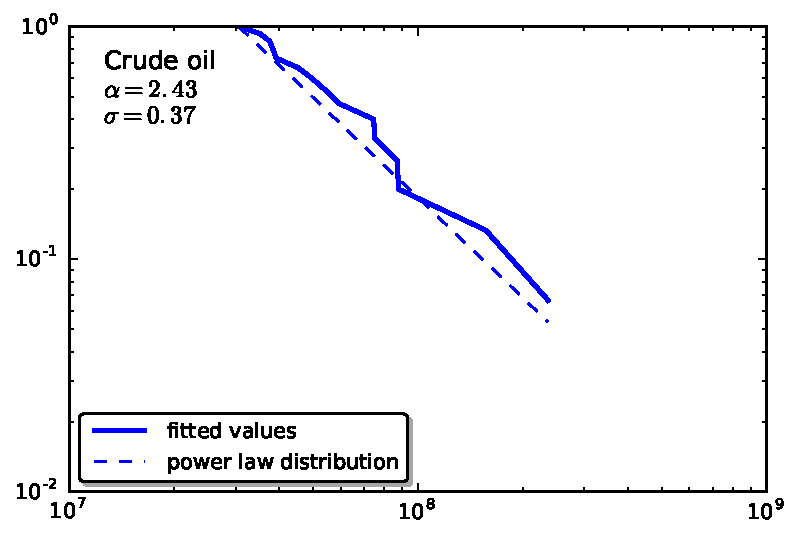
\includegraphics[width=\textwidth]{plots/oil_ccdf.pdf} 
  \caption{Crude Oil: 270900}
  \end{subfigure}
  \begin{subfigure}[b]{0.65\textwidth}
  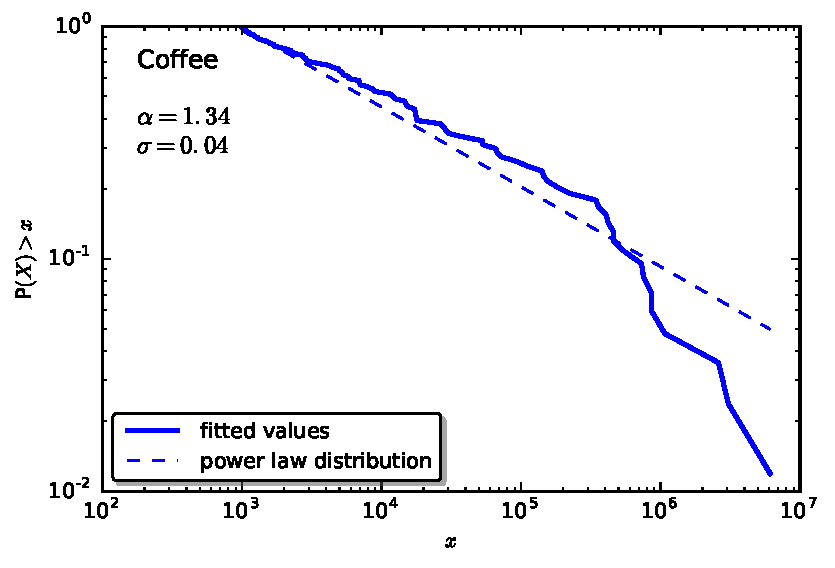
\includegraphics[width=\textwidth]{plots/coffee_ccdf.pdf} 
  \caption{Coffee: 090111}
  \end{subfigure}  \\
\footnotesize{$^*$CCDF: complementary cumulative distribution function.}
\end{figure} 


\subsection{Two econometric models} \label{models-econometric}
To test the theoretical relationship, I will use a variation on the empirical approach of Acemoglu, Akcigit, and Kerr, which is the analog to equation \ref{eq:main_aak}, and specified as follows:

\begin{equation} \label{eq:aak_analog}
\Delta \ \text{ln} \ Y_{i,t} = \delta_t + \psi \Delta \ \text{ln} \ Y_{i,t-1} + \beta^{own}Shock_{i,t-1} + \beta^{upstream}Shock_{i,t-1} + \varepsilon_{i,t}
\end{equation} 

where $\delta_t$ is the time fixed effect and $\varepsilon_{i,t}$ is the error term. The previous period output growth, previous period domestic shocks, and previous period upstream shocks determine the current period output fluctuation.

While my theoretical model is only slightly modified from that of Acemoglu, Akcigit, and Kerr, additional changes will be needed to estimate how domestic and upstream shocks affect output using international trade data. For the estimating equation \ref{eq:aak_analog} to fit with my hypothesis and the available data, two econometric models are identified in the following sections; both seek to estimate changes in each country's exports from own and upstream shocks. The first decomposes each country's previous period imports to identify inputs associated with upstream shocks with localized origins. The second model treats the price of oil as the exogenous shock. 

\subsubsection{Imports decomposition model} \label{imports_decomp}

The imports decomposition model seeks to explain fluctuations in the real value of exports, $X_{it} - X_{it-1}$, for country $i$, based on the composition of its imports. The model additionally seeks to incorporate own shocks as the previous history of exports as well shifts in the real effective rate of exchange between countries. Specifics of the model are included in this section.

The dependent variable is the change in the natural log of constant price exports of goods of country $i$ in time $t$, given by $\hat{x}_{it} = ln(X_t) - ln(X_{t-1})$. Changes to exports offer insight into the downstream pass-through of an upstream (and in this case cross-border) supply shock. That is, a supply shock to a trading partner will have various domestic effects on consumption baskets and prices, but this work argues that to get to the heart of whether shocks average out or propagate, one should look at whether the downstream is affected.

Next, to capture own (domestic) shocks, I control for changes to exchange rates and relative prices, as measured by the previous period change to the real effective exchange rate, $\hat{q}_{t-1}$. This is a domestic determinant of exports that is not correlated with the measures of network structure applied next.

Lastly, to test the hypothesis that the distribution of exporter sizes affects whether supply shocks propagate or die out, it is critical to measure the upstream (foreign) shock and isolate different shocks by the network structure through which they arrive. This can be done by decomposing previous period intermediate\footnote{All final consumption are goods excluded to isolate products which can have downstream affects} goods imports into four categories, defined as follows:

\begin{table}[ht]\centering \caption{Categories of intermediate good imports, goods indexed by $k$ \label{mtab}}
	\begin{tabular}{l | c | c}
	\toprule
	 & central players & no central players \\
	 \midrule
	 shock in time $t$ & $M^{cs}_{i,t-1} = \sum_{k=1}^{n} M^{cs}_{k,i,t-1}$ & $M^{ns}_{i,t-1} = \sum_{k=1}^{n}M^{ns}_{k,i,t-1}$ \\
	 \midrule
	 no shock & $M^{cn}_{i,t-1} = \sum_{k=1}^{n} M^{cn}_{k,i,t-1}$ & $M^{nn}_{i,t-1} = \sum_{k=1}^{n}M^{nn}_{k,i,t-1}$ \\
	 \bottomrule
	\end{tabular}
	\end{table}
	
where $M$ is the real US dollar value of imports to country $i$ from all other countries, and $m$ is its natural log.

While the empirical focus is variation of the decomposition of imports by country, a useful summary statistic for building understanding of the model is the decomposition of world imports of intermediate goods by year (figure 4). The vast majority of trade involves goods which do not feature power-law distributed exporter shares and are not subject to supply shocks from large natural disasters. Critically, the model aims to predict a country's fluctuation in next period output from the relative current imports of goods with power-law distributed suppliers and supply shocks.

\begin{figure} \label{fig:tot_decomp}
  \caption{Decomposition of world imports of intermediate goods}
  {\centering
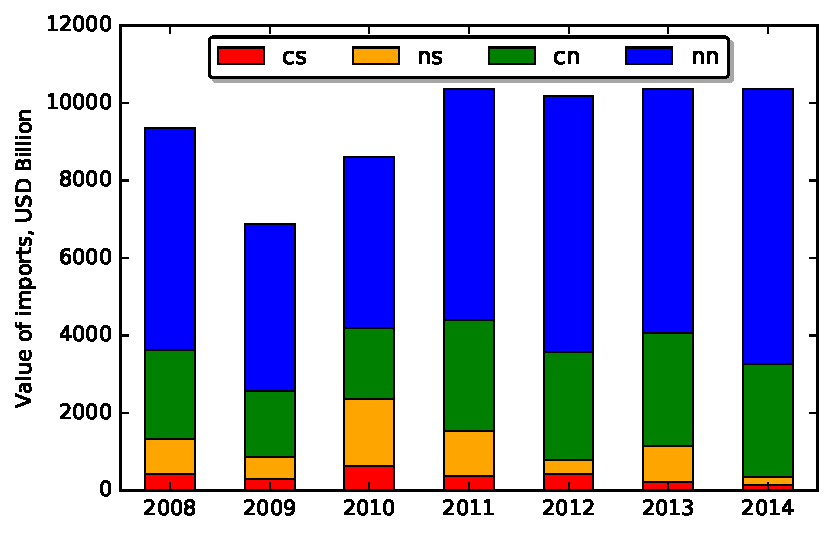
\includegraphics[scale=0.8]{plots/tot_decomp.pdf} \\
\footnotesize{Data source: CEPII BACI; own calculations. \\
Notes: Includes goods classified as intermediate by BEC. The series `cs' contains imports of goods with power-law distributed exporter sizes and a supply shock from a large natural disaster; `ns' includes goods with normally distributed exporter sizes and a supply shock; `cn' comprises goods with power-law distributed exporters and no supply shock to the exporting country; and `nn' is goods with normally distributed exporters and no supply shock.}}
\end{figure}

Combining the pieces of the imports decomposition model, I aim to estimate the following equation:

\begin{equation} \label{eq:decomp_est}
\hat{x}_{i,t} = \delta_{t} + \beta_1 \hat{x}_{i,t-1} + \beta_2 \hat{q}_{i,t-1} + \beta_3 m^{cs}_{i,t-1} + \beta_4 m^{ns}_{i,t-1} + \beta_5 m^{cn}_{i,t-1} + \varepsilon_{i,t}
\end{equation}

where $\delta_t$ is again the time fixed effects. The second and third terms attempt to control for domestic shocks. Previous period export growth, $\hat{x}_{i,t-1}$,  is unrelated to a next period supply shock, as is the previous period change in real effective exchange rate, $\hat{q}_{i,t-1}$. The variable of interest, which I hypothesize affects exports of downstream countries, is the previous period ($t-1$) log imports of goods with power law distribution exporter sizes when there has been a shock to the production of that good in period $t$, given by $m^{cs}_{i,t-1}$. To control for the possibility that the supply-shock, regardless of exporter sizes, causes the full adjustment in exports, the non-power-law-distributed imports from supply shock countries are included as $m^{ns}_{i,t-1}$. Lastly, to control for the possibility that exporter size distribution affects exports regardless of supply shocks, imports of goods where the exporter country sizes follow a power law distribution are included as $m^{cn}_{i,t-1}$.

My hypothesis is then:

\begin{align*}
\text{H}_0 &: \beta_3 < \beta_4, \quad \text{where:} \ \beta_3 < 0; \\
\text{H}_a &: \beta_3 \geq \beta_4 
\end{align*}

That is, I expect the coefficient on previous period imports of goods with power-law distributed exporter sizes that are imported from a country with a large natural disaster in the next period to be negative and more negative than the coefficient on natural disaster country imports that do not follow power-law distributed firm sizes. Results of estimation of equation \ref{eq:decomp_est} by fixed effects within ordinary least squares (OLS) and generalized method of moment (GMM) techniques is presented in section \ref{results_mdecomp}.

\subsubsection{Oil price shocks model} \label{models-oil}
The second model focuses on the role of one specific good, crude oil, in the propagation of shocks through network effects. The critical role of oil in economic activity has been well documented. Hamilton (1983, 2003) describes the role oil shocks plays in the broader economy, noting critically the nonlinear relation between oil prices and output growth. Through foundations in microeconomics, section \ref{modelsmicro} identifies domestic shocks and network effects as determinate of fluctuations in output. In the previous model, I decompose individual product imports by trade partner supply shock and product supplier size distributions to identify the role of exogenous shocks in domestic disturbances. The oil price shocks model instead assumes all network effects shocks to be conveyed by shocks to the price of oil and a country's connections to other countries.


\begin{figure}
  \caption{Total exports and the price of oil}
  \centering
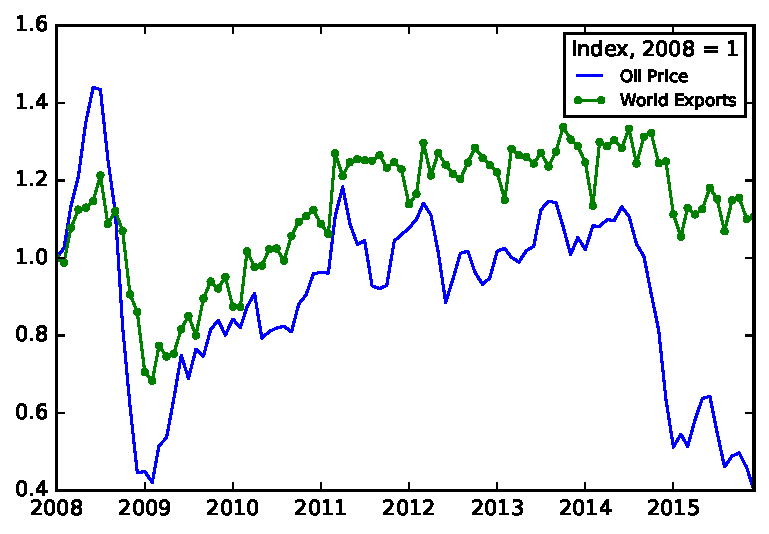
\includegraphics[scale=0.8]{plots/wti_ix.pdf} \\
\footnotesize{Source: IMF IFS and Primary Commodity Price Index.}\\
\end{figure}


The price of crude oil is determined globally by supply and demand and not fully within any one set of borders, and therefore can be considered exogenous. While oil is component in transportation, and therefore trade costs, the use in this model of the oil price is to reflect external shifts in supply and demand. That is, while a reduction of oil prices may lower trade costs, it is thought to reflect a reduction in global demand and therefore to precede reduced trade. The oil price shock measure, which is high-frequency and not location-specific, is applied to monthly data on total trade, from the IMF's Direction of Trade Statistics (DOTS). As new information is obtained and changes to the price of oil are revealed, the following estimation equation seeks to identify how different exporters respond in the very short-run:
\begin{equation}
\hat{x}_{i,t} = \alpha_{i} + \beta_1 x_{i,t-1} + \beta_2 \hat{q}_{i,t-1} + \beta_3 (c^e_{i,t-1} \times \hat{\rho}_{t}) + \varepsilon_{i,t}
\end{equation}

where $\alpha_{i}$ is the country specific fixed effect, $c^e_{i,t}$ is the eigenvector centrality of imports and $\hat{\rho}_{t}$ is the recent month change in the price of crude oil. As discussed in section \ref{nw3}, this centrality term follows a similar algorithm to the PageRank algorithm used by Google, where, in the case of imports, the number and size of import flows is important, but the relative importance of your suppliers is also taken into consideration. The term is meant to measure how influential each country is in each month to the global consumption of intermediate goods, with particular focus on the relative importance of its suppliers. A high eigenvector centrality score is associated with a strong reliance on imports of intermediate goods from influential suppliers. Countries with a high score are expected to 1) have export fluctuations more closely tied to network effects, and therefore 2) propagate exogenous shocks.

Estimated eigenvector centralities are largely stable over time, especially in the very short run, for the vast majority of countries. However, this calculation still allows for interesting examination of how each country's influence in the global trade network has gradually changed. Figure 9 in the appendix maps change in the eigenvector centrality score of exports and imports for each country since 2008. These figures show a shift in influence away from Europe and towards China, Korea, Vietnam, Mexico, and others. The average eigenvector centrality scores of exports by continent confirm the shift of influence away from Europe (figure 6).

This model is primarily interested in the interaction of a country's position in the network with exogenous shocks to supply and demand, captured through the price of oil. The estimating equation therefore calculates the interaction between the centrality term and the oil price term as representative of the network effects identified in equation \ref{eq:main_aak}. The interaction term is meant to capture the mechanism through which an exogenous shock enters (the centrality to global imports) and the exogenous shock itself (a change in oil prices). As in the previous model, and as shown in equation 7, the point of measurement is changes to each country's exports. 

If exogenous shocks are indeed amplified by a country's role in the network, for example through its integration in global value chains, the coefficient on the interaction term will be positive and significant, even in the very short-run. The presence of high-frequency volatility in exports from network effects would suggest countries more integrated in global trade experience a larger change in real exports from exogenous shocks.

\subsection{Data sources and treatment} \label{data_sources}
The imports decomposition model relies on dis-aggregated international trade data at the product level, which is obtained through the BACI dataset produced by CEPII. Specifically, the data used follow the 2007 version of the harmonized system (HS2007) and are aggregated at the six-digit level. BACI provides a cleaned and expanded version of UN Comtrade data, and importantly also removes re-exports and re-imports. The dataset includes annual observations of trade value in thousands of US Dollars and trade volume in metric tons from 2007 to 2014 on 217 countries and self-governing entities. The BACI dataset covers more than 5200 products per year, and includes both intermediate goods and final consumption goods. The Broad Economic Categories (BEC) are used to identify which are intermediate goods and to exclude final consumption goods from the sample, bringing the total to 3805 goods. 

Exogenous supply shocks in the import decomposition model are identified from global information on natural disasters. These disasters are classified by type, location, and date using the EM-DAT international disasters database. Disasters between 2008 and 2015 are initially grouped by year and country, however the database is very extensive, and this research is focused primarily on large exogenous supply shocks from natural disasters. To capture only large disasters (those with potential cross-border implications), only those which result in a loss of 40 or more lives are included in the sample, bringing the period total to 153 disasters.

The oil price shocks model focuses instead on higher-frequency changes to trade of all goods. Therefore, data on international trade is obtained from the IMF's Direction of Trade Statistics (DOTS), with monthly observations from 2008 to 2015 for 183 countries. The oil price shocks model relies on the monthly average change in the U.S. Dollar price of West Texas Intermediate (WTI) crude oil as the measure of exogenous shocks. Oil price data is obtained from the IMF's Primary Commodity Prices dataset. 

Remaining data on total exports of goods, import and export prices, and the real effective exchange rate (REER) for both models are obtained from the IMF's International Financial Statistics (IFS). The value of total exports for each country is measured free on board\footnote{The oil price shocks model measures this flow from the importer's perspective for accuracy, where the exporter covers costs, insurance, and freight.}, and adjusted for changes to the export price index of each country\footnote{In a few cases, the regional export or import price index is used.}. Values obtained from the decomposition of imports are also adjusted for changes in prices, using the import price index of the importer country. The REER is obtained as an index, and captures trade-partner weighted changes in exchange rates and relative price levels. 

The availability of sufficient exchange rate, exports, and price information is limited, reducing the total number of countries included in econometric analysis of the imports decomposition model to 80. The imports decomposition and product-level analysis, however, is based on the full sample of 217 countries, so that the fewest possible nodes are excluded from the network analysis stage.

\section{Results} \label{results}
This section presents the main findings of the network analysis components, the specific case of oil and gas networks, and both models for examining broader implications of network structure. Results largely confirm intuitive expectations discussed in section 4. The finding related to model one are significant both economically and statistically, whereas results from model two are far less robust, suggesting that network effects do not present themselves fully in the very short-run.

\subsection{Results: Network analysis} \label{results_nw}
First, a brief discussion of the main findings in the estimation of degree distribution by product and eigenvector centrality by country. Beyond the estimation of changes to exports, the network analysis components of this work offer interesting insight into which products have power-law distributed exporters and how countries' roles in international trade have changed.

The out-degree distribution calculated for each product in each year identifies certain categories of products are having an outsized share of power-law distributed suppliers. Figure 6 presents a summary for 2014 of the representation of broad economic categories of intermediate goods in the full sample and in the power-law distributed goods category. Industrial supplies represent the most traded category in the full sample but are under-represented in the power-law distributed sample. The fuels and lubricants category claims 60\% of the trade of all power-law distributed goods. Food and beverage and industrial transport equipment are strongly under-represented among power-law distributed goods. 

In terms of individual goods, by value of 2014 exports, oil and gas are the largest power-law distributed goods. Additional power-law distributed goods with large trading volumes include cathodes, copper ore, electrical component boards, and medical instruments (table 5). Normally distributed goods include gold, various types of automobiles, cellular telephones, laptop computers, and electronic integrated circuits (table 6). 

At a country level, China is shown to be both the largest exporter in real terms and the most influential exporter by eigenvector centrality, in all years. The United states is second in both categories, and, like China, has seen a growing eigenvector centrality of exports (table 4). Eigenvector centrality scores for most of Europe have fallen since 2008, while emerging market countries, especially those less dependent upon primary commodity exports, such as China, Korea, Singapore, and Vietnam have seen large increases in eigenvector centrality scores for exports. 

\begin{figure}
  \caption{Intermediate product exports by category, 2014}
  \centering
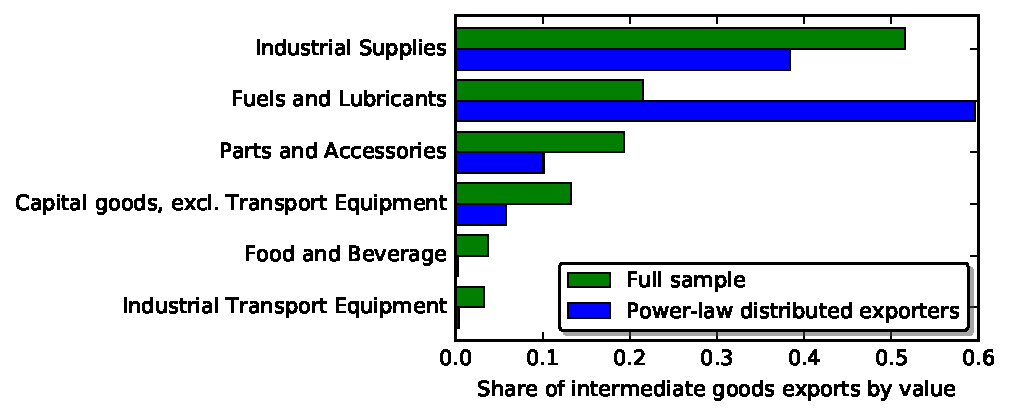
\includegraphics[scale=0.7]{plots/bec_cat.pdf} \\
\footnotesize{Source: CEPII BACI; BEC; own calculations.}\\
\end{figure}

\subsection{Results: Oil and gas in detail} \label{results_oil_gas_detail}
Next, results surrounding the most influential power-law distributed products, crude oil and natural gas, are discussed in further detail. As discussed in section \ref{nw4}, crude oil is the most traded good on earth and features a very public group of suppliers who work together (prima facie) to determine global supply. In practice however, suppliers of oil and gas are extremely vulnerable to shifts in global demand. 

Evidence since 2010 suggests a worldwide growth of renewable energy, a shift towards lower energy intensity in developed countries, and very low, unbalanced, and often negative growth in access to electricity in the least developed countries (World Bank 2015). These developments all factor negatively into the global demand for oil and gas, which can partially explain low prices. Additionally, important changes to the supply of natural gas, which has substitution effects with other energy sources, include advancements in horizontal drilling and hydraulic fracturing. The natural gas supply developments both shifts the location of production, dramatically increasing domestic production in the United States (Wang et al 2014) and other countries, and changes the dynamics for how energy supply responds to changes in prices. Technological developments have shortened the time required to increase the production of natural gas, if, for example, prices increase.

The combined effect of recent developments in the production and demand for oil and gas has resulted in a gradual decline in the estimated power law exponent parameter for oil and a somewhat volatile increase in the estimated parameter for natural gas. Additionally, the geographic changes in production are partially documented through analysis of the trade network (figure 8). The U.S. claims a decreasing share of imports, while the more-advanced emerging market shares have increased, particularly the share of China in the global imports of oil. In general, import shares of natural gas are falling in many European countries as energy production has become more localized and renewable sources become more competitive.

\subsection{Results: Imports decomposition model} \label{results_mdecomp}

Three variations of the estimating equation were applied to a balanced panel of data covering 80 countries, with annual observations during 2008--2015. The first variation excludes the previous period real exports as a control variable. The second variation of the estimating equation includes the previous period log-level of real exports as a control, and the third variation includes lagged export growth to generate a dynamic panel. All three variations estimate coefficients in line with the hypothesis presented in section \ref{imports_decomp}. 

The estimated coefficients are presented in Table \ref{tab:ImportDecompModel}. The first two columns present the fixed-effects within OLS regression estimates, while the last two columns present the one-stage generalized method of moments (GMM) estimates. In all three models, the variable of interest, the previous period imports of goods with central suppliers from supply shock countries ($m^{cs}$), is shown to be negative and statistically significant. Each log unit of $m^{cs}$ is estimated to reduce exports by between 2 and 5 percent in the following year, offering evidence that supply shocks can be transmitted internationally through goods with power-law distributed suppliers. Supply shocks do not seem to transmit through goods with normally distributed exporter sizes, even though these goods ($m^{ns}$) are imported from countries with a supply shock. Theoretically, in these cases alternate suppliers are readily available. An increased level of $m^{ns}$ is actually shown to increase exports, with statistical significance varying by model. 

\begin{table}[!htb]\centering
 \caption{Estimation results: Import decomposition model
\label{tab:ImportDecompModel}}
\begin{tabular*}{0.8\textwidth}{@{\extracolsep{\fill}}lccc}		
Export growth$_t$ ($\hat{x}_{it}$)	& \multicolumn{2}{c}{Fixed-effects within OLS} &	\multicolumn{1}{c}{GMM} \\
\cline{2-4}			
	& \multicolumn{1}{c}{(1)\mbox{\ }} &	\multicolumn{1}{c}{(2)\mbox{\ }} &	\multicolumn{1}{c}{(3)} \\
\hline			
Export growth$_{t-1}$ &	&	 &	-.180\\
\quad $\hat{x}_{it-1}$ &	&	 &	\raisebox{.7ex}[0pt]{\scriptsize (0.111)}\\
Exports$_{t-1}$ &	&	-.495 &	 \\
\quad $x_{it-1}$ &	&	\raisebox{.7ex}[0pt]{\scriptsize (0.041)$^{***}$} & 	 \\
REER change$_{t-1}$ &	-.123 &	-.009 &	-.339 \\
\quad $\hat{q}_{it-1}$ &	\raisebox{.7ex}[0pt]{\scriptsize (0.158)} &	\raisebox{.7ex}[0pt]{\scriptsize (0.139)} &	\raisebox{.7ex}[0pt]{\scriptsize (0.147)$^{**}$} \\
\textbf{Imports$_{t-1}$: pld, shock} &	\textbf{-.040} &	\textbf{-.021} &	\textbf{-.050} \\
\quad $m^{cs}_{it-1}$ &	\raisebox{.7ex}[0pt]{\scriptsize (0.011)$^{***}$} &	\raisebox{.7ex}[0pt]{\scriptsize (0.01)$^{**}$} &	\raisebox{.7ex}[0pt]{\scriptsize (0.026)$^{*}$} \\
Imports$_{t-1}$: no pld, shock &	0.029 &	0.051 &	0.048 \\
\quad $m^{ns}_{it-1}$ &	\raisebox{.7ex}[0pt]{\scriptsize (0.017)$^{*}$} &	\raisebox{.7ex}[0pt]{\scriptsize (0.015)$^{***}$} &	\raisebox{.7ex}[0pt]{\scriptsize (0.019)$^{**}$} \\
Imports$_{t-1}$: pld, no shock &	-.076 &	0.017 &	-.056 \\
\quad $m^{cn}_{it-1}$ &	\raisebox{.7ex}[0pt]{\scriptsize (0.023)$^{***}$} &	\raisebox{.7ex}[0pt]{\scriptsize (0.022)} &	\raisebox{.7ex}[0pt]{\scriptsize (0.061)} \\
Year dummies &	yes &	yes &	yes \\
\hline
Observations &	560 &	560 &	480 	\\
Countries & 80 & 80 & 80 \\
Adjusted $R^2$ &	0.65  &	0.73 &	\\
Hansen p-value & & & 0.07 \\
AR(1) & & & 0.01 \\
AR(2) & & & 0.44\\
Instruments & & & 31 \\
\hline\hline					
\multicolumn{4}{l}{\footnotesize{Standard errors in parenthesis.}}\\
\multicolumn{4}{l}{\footnotesize{Significance levels
:\hspace{1em} $^{*}$ : 10\% \hspace{1em}
$^{**}$ : 5\% \hspace{1em} $^{***}$ : 1\% \normalsize}}
\end{tabular*}
\end{table}			

The results are considered economically significant in that the type of intermediate goods that a country imports affects how it responds to exogenous supply shocks elsewhere. This result provides an argument for diversification of inputs by location and type. While, as seen in figure 4, the $m^{cs}$ share of all imports is quite small, the decomposition revealed concentrated and shifting pockets of large volumes of these negative network effect imports. 

The domestic shocks to exports captured by previous period export values are shown to be statistically significant and may be capturing trends such as a convergence in export growth rates. The previous period changes to the real effective exchange rate are shown to be statistically significant only in the third variation of the model. An increase in the real effective exchange rate makes exports relatively more expensive and results in an inward shift in aggregate demand, putting downward pressure on export growth.

\subsection{Results: Oil price shocks model} \label{results_oil}

Estimation results for the oil price shocks model are somewhat consistent with the hypothesis that shocks transmitted through central suppliers are propagated. The results, however, are not robust nor offer much explanatory power in the very short run. Additionally, the centrality scores vary little over time, and therefore are not well specified in a model with time fixed effects. 

The estimated coefficients for the oil price shocks model are presented in table \ref{tab:ImportDecompModel}. The first three columns present the fixed-effects within OLS regression estimates, while the last columns presents the common correlated effects (CCE) mean group estimation results. The CCEMG model is used due to the long time series of the panel, and allows for country- and time-specific constant terms. In this model, the independent variable of interest, the interaction term between centrality and oil price shocks, shows statistically significant propagation of the oil price shock. However, the economic significance is unclear and requires further discussion. 

All four variations of the oil price shocks model equation return an estimated negative effect of previous period export levels to current growth rates, as seen in the previous model. The panel time series model, variation 4, predicts the opposite sign of what is expected for changes to the real effective exchange rate. The oil price shock itself is found to have a positive coefficient on current export growth, as expected in discussion of variable selection. It's important to note here the potential endogeneity issue of using oil prices to estimate changes in real exports. As discussed in section \ref{results_oil}, the supply, and therefore exports, of oil respond positively to changes in price. That is, oil exports are increased in response to a positive oil price shock and decreased in response to a negative price shock. The theoretical support for oil as an exogenous shock may not hold when the point of measurement is exports. 

\begin{table}[!htb]\centering
\caption{Estimation results ($\hat{x}_{it}$): Oil price shocks model
\label{tab:OilShocksModel}}
\begin{tabular*}{0.8\textwidth}{@{\extracolsep{\fill}}lcccc}				
Export growth$_t$ ($\hat{x}_{it}$)	& \multicolumn{3}{c}{Fixed-effects within OLS} &	\multicolumn{1}{c}{CCEMG} \\
\cline{2-5}				
	& \multicolumn{1}{c}{(1)\mbox{\ }} &	\multicolumn{1}{c}{(2)\mbox{\ }} &	\multicolumn{1}{c}{(3)\mbox{\ }} &	\multicolumn{1}{c}{(4)} \\
\hline				
Exports$_{t-1}$ &	-.118 &	-.118 &	-.116 &	-.528 \\
\quad $x_{it-1}$ &	\raisebox{.7ex}[0pt]{\scriptsize (0.007)$^{***}$} &	\raisebox{.7ex}[0pt]{\scriptsize (0.007)$^{***}$} &	\raisebox{.7ex}[0pt]{\scriptsize (0.007)$^{***}$} &	\raisebox{.7ex}[0pt]{\scriptsize (0.029)$^{***}$} \\
REER change$_{t-1}$ &	0.122 &	0.093 &	0.096 &	0.472 \\
\quad $\hat{q}_{it-1}$ &	\raisebox{.7ex}[0pt]{\scriptsize (0.091)} &	\raisebox{.7ex}[0pt]{\scriptsize (0.09)} &	\raisebox{.7ex}[0pt]{\scriptsize (0.09)} &	\raisebox{.7ex}[0pt]{\scriptsize (0.117)$^{***}$} \\
oil price shock$_{t-1}$ &	&	0.353 &	0.356 &	\\
\quad $\hat{\rho}_{t}$ &	&	\raisebox{.7ex}[0pt]{\scriptsize (0.024)$^{***}$} &	\raisebox{.7ex}[0pt]{\scriptsize (0.024)$^{***}$} &	\\
export centrality$_{t-1}$ &	&	&	-.515 &	\\
\quad $c_{it-1}$&	&	&	\raisebox{.7ex}[0pt]{\scriptsize (0.196)$^{***}$} &	\\
\textbf{(centrality $^*$ shock)} &	\textbf{1.215} &	&	&	\textbf{9.691} \\
\quad $(c_{it-1} \times \hat{\rho}_{t})$&	\raisebox{.7ex}[0pt]{\scriptsize (0.193)$^{***}$} &	&	&	\raisebox{.7ex}[0pt]{\scriptsize (3.788)$^{**}$} \\
\hline
Observations &	5076 &	5076 &	5076 &	5076 \\
Countries &	94 &	94 &	94 &	94 \\
Adjusted $R^2$ &	0.05 &	0.081 &	0.082 &	\\
Trends stat. sig. &	&	&	&	0.556 \\
\hline\hline	
\multicolumn{5}{l}{\footnotesize{Standard errors in parenthesis.}}\\
\multicolumn{5}{l}{\footnotesize{Significance levels
:\hspace{1em} $^{*}$ : 10\% \hspace{1em}
$^{**}$ : 5\% \hspace{1em} $^{***}$ : 1\% \normalsize}}					
\end{tabular*}%				
\end{table}

As mentioned, there are doubts to the reliability and economic significance of the estimates of the second model. While initial consideration shows some propagation of network effects from centrality, which is expected, the variance of estimates for this parameter, as well as the lack of explanatory power and the unexplained sign on the REER coefficient, suggest issues with model specification. Additionally, while this model intentionally attempts to capture very short-run effects, it is clear that the production process for many goods is longer than the one month rate of change explored in this model.  

As a result, rather dismiss the possibility of a very short run response to global shocks determined by network position, additional work is required to fully explore the possibility, and the overall results obtained by this model should not be interpreted as economically meaningful. 

\section{Conclusion} \label{conclusion}
Model 1 results discussed in section \ref{results} are largely consistent with the theoretical prediction that a country's role in its network, and the size distribution and role of its trading partners, determines its exposure to routine exogenous shocks. Indeed, even at an international level, the distribution of supplier sizes presents a mechanism through which localized shocks can cross borders. Beyond the implication for international trade as a whole, one key contribution of this work is the discussion of international trade networks for individual goods. Additionally, this finding generates several policy implications, as well as the need for further research, which are discussed in this section. 

As demonstrated, the global trade network for individual goods varies both between goods and over time, and network analysis can succinctly capture these variations. Oil and gas trade networks have shifted in response to broad changes in energy production and consumption, and these changes can be seen in detail (figure 7, for example). The same process works for any product and while writing this paper many interesting cases were considered. Several products identified in literature related to global value chains and the 2011 natural disasters in Japan and Thailand (discussed in section \ref{modelstheory}) show power-law distributed suppliers before the disasters and a less central role for Japan and Thailand following the disasters. The examination of trade networks at a product level may be able to identify certain `linchpin' products based on their unique characteristics.

Additional key implications from this work are primarily related to trade and exchange rate policies. First, the network of importers and exporters for each country is partially determined by the tariff rates it offers to partners. Many countries have zero or near-zero tariff rates for a selected subgroup of partners, which creates opportunities for strategic collaboration, but can also lead to situations where only the inputs from a small set of countries are competitive, and comparable inputs from other countries are prohibitively expensive. By artificially selecting which geographic areas are competitive, a country may expose itself to risks from shocks to its few suppliers. 

Of course, the shocks described in the first model of this paper are inevitable. However, the tools available to countries to respond to shocks differ. Regional integration has reduced the number of independent currencies, and essentially centralizes an otherwise localized tool for adjusting to localized shocks. Countries that are able to adjust their exchange rate may be able to use the tool to secure inputs from alternative suppliers that are not prohibitively expensive. While the models in this paper do not observe domestic effects directly, the same models could be applied to a vector of domestic dependent variables to further understanding of domestic policy responses.

There are several other extensions. Work should be done to identify the causes of a country's eigenvector centrality in international trade. Potential areas for exploration include currency and exchange rate considerations, and actual tariff rates by partner country and product. For example, how do changes to the the ability of a country to adjust the exchange rate of its currency affect its role in global trade. Likewise, how do bilateral and multilateral trade liberalization efforts and regional trade agreements affect the composition of trade partners, as measured by their relative importance.

I also advocate further work within the topic of this paper. Primarily, additional work could address endogeneity concerns with the oil price shocks model, perhaps through estimation of dynamic correlations, and also to include a model which examines network changes in trade when a central supplier itself experiences a natural disaster. 


\newpage



\begin{thebibliography}{99}
\bibitem{acemoglu-2016} 
Daron Acemoglu, Ufuk Akcigit, and William Kerr (2016)
Networks and the Macroeconomy: An Empirical Exploration. 
Chapter in NBER book NBER Macroeconomics Annual 2015, Volume 30, Martin Eichenbaum and Jonathan Parker, editors, 276--335.

\bibitem{acemoglu-2012} 
Daron Acemoglu, Vasco M. Carvalho, Asuman Ozdaglar \& Alireza Tahbaz-Salehi (2012) The Network Origins of Aggregate Fluctuations. Econometrica 80(5), 1977--2016.

\bibitem{an}
Haizhong An, Weiqiong Zhong, Yurong Chen, Huajiao Li \& Xiangyun Gao (2014) Features and evolution of international crude oil trade relationships: A trading-based network analysis. Energy, 74(), 254--259. 

\bibitem{bonacich}
Phillip Bonacich (1972) Factoring and Weighted Approaches to Status Scores and Clique Identification. Journal of Mathematical Sociology. 2, 113--120.

\bibitem{canis}
Bill Canis (2011) The Motor Vehicle Supply Chain: Effects of the Japanese Earthquake and Tsunami. CRS Report for Congress. Congressional Research Service. May 23, 2011.

\bibitem{carvalho}
Vasco M. Carvalho (2014) From Micro to Macro via Production Networks. Journal of Economic Perspectives 28(4), 23--48.

\bibitem{chaney}
Thomas Chaney (2014) The network structure of trade. American Economic Review, 104(11), 3600--3634.

\bibitem{clauset}
Aaron Clauset, Cosma Rohilla Shalizi, \& M. E. J. Newman (2009) Power-Law Distributions in Empirical Data. SIAM Review, 51(4), 661--703.

\bibitem{alatriste}
Martha G. Alatriste Contreras and Giorgio Fagiolo (2014) Propagation of economics shocks in input-output networks: A cross-country analysis. Physical Review, 90(), 062812-1--9. 

\bibitem{debenedicis}
De Benedictis and Lucia Tajoli (2011) The World Trade Network. The World Economy, 34(8), 1417--1454.  

\bibitem{fagiolo}
Giorgio Fagiolo, Javier Reyes \& Stefano Schiavo (2009) The evolution of the world trade web: a weighted-network analysis. Journal of Evolutionary Economics, 20(4), 479--514.

\bibitem{fuller}
Thomas Fuller (2011) Thailand Flooding Cripples Hard-Drive Suppliers. New York Times. Global Business, November 6, 2011.

\bibitem{gabaix-2011} 
Xavier Gabaix (2011) The Granular Origins of Aggregate Fluctuations. Econometrica 79(3), 733--772.

\bibitem{gabaix-2016} 
----- (2016) Power Laws in Economics: An Introduction. Journal of Economic Perspectives, 30(1), 185--206.

\bibitem{geng}
Jiang-Bo Geng, Qiang Ji, Ying Fan (2014) A dynamic analysis on global natural gas trade network. Applied Energy, 132(), 23--33.

\bibitem{glickrose}
Reuven Glick and Andrew K. Rose (1999) Contagion and trade Why are currency crises regional? Journal of International Money and Finance 18 (4) 603--617.

\bibitem{hamilton1}
James D. Hamilton (1983) Oil and the Macroeconomy since World War II. Journal of Political Economy, 91(2), 229--248.

\bibitem{hamilton2}
----- (2003) What is an oil shock? Journal of Econometrics, 113, 363--398.

\bibitem{hruska}
Joel Hruska (2013) Two years later, HDD prices settle back to normal. Extreme Tech, November 27, 2013. 

\bibitem{imf}
International Monetary Fund (2011) Changing Patterns of Global Trade. IMF Policy Paper, June 15, 2011.

\bibitem{jackson}
Matthew O. Jackson (2008) Social and Economic Networks. Princeton University Press.

\bibitem{Jovanovic}
Boyan Jovanovic (1987) Micro Shocks and Aggregate Risk. The Journal of Quarterly Economics, 102(2), 395--410.

\bibitem{kalimendezreyes}
Raja Kali, Fabio M\'endez \& Javier Reyes (2007) Trade structure and economic growth. The Journal of International Trade \& Economic Development, 16(2), 245--269.

\bibitem{kalireyes}
Raja Kali and Javier Reyes (2007) The Architecture of Globalization: A Network Approach to International Economic Integration. Journal of International Business Studies, 38(4), 595--620.

\bibitem{kydland}
Finn R. Kydland and Edward C. Prescott (1982) Time to Build and Aggregate Fluctuations. Econometrica 50(6), 1345--1370.

\bibitem{lohr}
Steve Lohr (2011) Stress Test for the Global Supply Chain. New York Times. Business Day, March 19, 2011. 

\bibitem{Loungani}
Prakash Loungani (1986), Oil Price Shocks and the Dispersion Hypothesis. Review of Economics and Statistics, 58, 536--539.

\bibitem{lucas} 
Robert R. Lucas, Jr. (1977) Understanding Business Cycles. Carnegie-Rochester Conference Series on Public Policy, 5, 7--29. 

\bibitem{minoiu}
Camelia Minoiu and Javier A. Reyes (2011) A network analysis of global banking: 1978-2009. IMF Working Paper, 11(74).

\bibitem{nemeth}
Roger J. Nemeth and David A. Smith (1985) International Trade and World-System Structure: A Multiple Network Analysis. Review (Fernand Braudel Center), 8(4), 517--560.

\bibitem{onder}
Ali Sina Onder and Hakan Yilmazkuday (2014) Trade Partner Diversification and Growth: How Trade Links Matter. Federal Reserve Bank of Dallas Globalization and Monetary Policy Institute, Working Paper No. 192, September. 

\bibitem{smith}
David A. Smith and Douglas R. White (1992) Structure and Dynamics of the Global Economy: Network Analysis of International Trade 1965-1980. Social Forces, 70 (4), 857--893

\bibitem{snyderkick}
David Snyder and Edward L. Kick (1979) Structural Position in the World System and Economic Growth, 1955-1970: A Multiple-Network Analysis of Transnational Interactions. American Journal of Sociology, 84(5), 1096--1126.

\bibitem{wang}
Qiang Wang, Xi Chen, Awadhesh N. Jha, \& Howard Rogers (2014) Natural gas from shale formation--The evolution, evidences and challenges of share gals revolution in United States. Renewable and Sustainable Energy Reviews, 30, 1--28.

\bibitem{worldbank}
World Bank (2015) Sustainable Energy for All 2015: Progress Toward Sustainable Energy. Washington, DC: World Bank.

\bibitem{zhang}
Dayong Zhang (2008) Oil shock and economic growth in Japan: A nonlinear approach. Energy Economics, 30, 2374--2390.

\bibitem{zhanghy}
Hai Ying Zhang, Qiang Ji \& Ying Fan (2014) Competition, transmission and pattern evolution: A network analysis of global oil trade. Energy Policy, 73 312--322.

\end{thebibliography} 


\newpage 
\setcounter{secnumdepth}{0}
\section{Appendix} \label{appendix}

\noindent \begin{table}[ht]\centering
 \caption{Measures of Real Exports by Country (25 largest exporters shown)}
 \resizebox{\textwidth}{!}{%
\begin{tabular}{lrrrccr}
\toprule
 &   & Real & Export  & Eigenvector & Eigenvector & Change in\\
 & 2015 Real & Export & Growth & Centrality & Centrality & Centrality \\ 
             & Exports &  Growth &  Volatility & of Exports & of Exports &  of Exports\\
Country Name &   USD, billion &   since 2008      &     ($\sigma^2(\bar{x}_{it})$) & Rank 2008 & Rank 2015 &   since 2008   \\
\midrule
China              & 2307.97 & 0.82  & 0.23 & 1  & 1  & 0.08  \\
United States      & 1514.26 & 0.34  & 0.17 & 2  & 2  & 0.02  \\
Germany            & 1224.68 & -0.14 & 0.20  & 3  & 3  & -0.04 \\
Japan              & 506.32  & -0.25 & 0.22 & 4  & 4  & -0.05 \\
France             & 467.13  & -0.15 & 0.20  & 8  & 8  & -0.04 \\
Italy              & 448.01  & -0.05 & 0.23 & 11 & 11 & -0.03 \\
United Kingdom     & 422.77  & -0.09 & 0.23 & 10 & 10 & -0.03 \\
Netherlands        & 391.46  & -0.20  & 0.26 & 7  & 9  & -0.05 \\
Belgium            & 369.06  & -0.14 & 0.24 & 12 & 14 & -0.04 \\
Canada             & 351.46  & -0.12 & 0.31 & 5  & 6  & -0.04 \\
Mexico             & 341.42  & 0.34  & 0.29 & 9  & 7  & 0.05  \\
Singapore          & 308.25  & 0.07  & 0.25 & 23 & 22 & 0.00  \\
Russian Federation & 303.69  & -0.16 & 0.38 & 14 & 15 & -0.04 \\
Spain              & 251.34  & -0.06 & 0.23 & 19 & 23 & -0.01 \\
Malaysia           & 201.93  & 0.32  & 0.25 & 15 & 12 & 0.01  \\
Switzerland        & 187.55  & 0.10   & 0.21 & 18 & 18 & 0.00  \\
Poland             & 177.32  & 0.24  & 0.24 & 30 & 26 & 0.00  \\
Czech Republic     & 149.28  & 0.21  & 0.23 & 31 & 28 & 0.00  \\
Brazil             & 149.09  & 0.03  & 0.38 & 17 & 17 & 0.00  \\
Australia          & 138.78  & 0.27  & 0.41 & 16 & 13 & 0.01  \\
Austria            & 137.91  & -0.12 & 0.22 & 25 & 27 & -0.01 \\
Saudi Arabia       & 135.28  & -0.37 & 0.66 & 13 & 19 & -0.05 \\
Sweden             & 117.68  & -0.38 & 0.26 & 28 & 31 & -0.02 \\
Norway             & 83.30    & -0.48 & 0.46 & 24 & 33 & -0.03 \\
Hungary            & 79.96   & -0.24 & 0.22 & 39 & 35 & 0.00 \\
\bottomrule 
\multicolumn{7}{l}{\footnotesize{Source: CEPII BACI; own calculations.}}\\
\end{tabular}}
\end{table}



\begin{figure}
  \caption{Average eigenvector centrality score of imports by continent}
  \centering
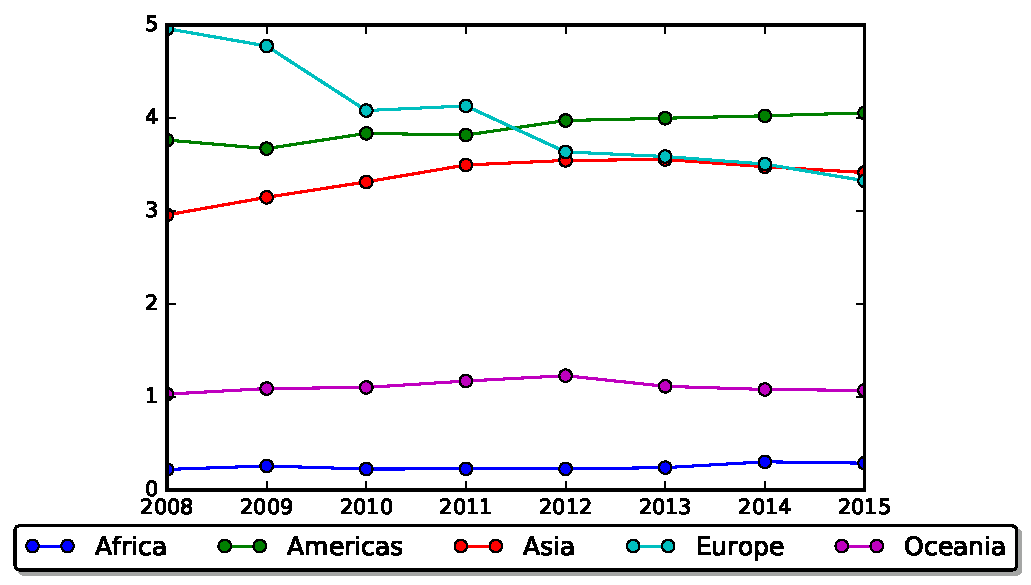
\includegraphics[scale=0.7]{plots/cent_continent.pdf} \\
\footnotesize{Source: CEPII BACI; own calculations.}\\
\end{figure}


\begin{table}[ht]
\centering
\caption{Top ten power-law distributed goods by export value, 2014}
\resizebox{\textwidth}{!}{%
\label{pldgoods}
\begin{tabular}{llllllll}
\toprule
HS    & USD value       & Quantity       & No. of   & No. of   & Estimated   & $\sigma$ of & \\
code    & exports & in tons       & exporters   & importers   & $\alpha$  & estimate & Product Name \\
\midrule
270900 & 14007.9 & 19936.2 & 116 & 141 & 2.43 & 0.36   & Crude oil                               \\
271121 & 1810.5  & 3889.3  & 65  & 96  & 2.17 & 0.33  & Natural gas                             \\
271111 & 1746.4  & 2514.9  & 63  & 98  & 2.18 & 0.34  & Natural gas                             \\
740311 & 617.8   & 93.8    & 78  & 94  & 2.61 & 0.41  & Cathodes                                \\
260300 & 536.2   & 238.2   & 83  & 81  & 2.22 & 0.36  & Copper ore                              \\
853710 & 477.7   & 6.4     & 192 & 213 & 2.14 & 0.24  & Electrical control boards               \\
732690 & 411.3   & 89.1    & 196 & 216 & 2.30 & 0.29  & Articles of iron/steel                  \\
901890 & 403.9   & 7.2     & 176 & 213 & 2.43 & 0.43  & Instruments: medical \\
854430 & 364.3   & 15.9    & 134 & 191 & 2.29 & 0.32  & Ignition wiring sets\\
840999 & 345.4   & 29.3    & 190 & 216 & 2.83 & 0.61  & Misc. engine parts\\
\bottomrule        
\multicolumn{7}{l}{\footnotesize{Source: CEPII BACI; own calculations.}}\\         
\end{tabular}}
\end{table}

\begin{table}[ht]
\centering
\caption{Top ten normally distributed goods by export value, 2014}
\resizebox{\textwidth}{!}{%
\label{normalgoods}
\begin{tabular}{llllllll}
\toprule
HS    & USD value       & Quantity       & No. of   & No. of   & Estimated   & $\sigma$ of & \\
code    & exports & in tons       & exporters   & importers   & $\alpha$  & estimate & Product Name \\
\midrule
710812 & 2876.9  & 0.3     & 145 & 120 & 1.80  & 0.14  & Gold \\
870323 & 2705.7  & 225.3   & 191 & 215 & 1.21  & 0.02  & Medium sized cars \\
851712 & 2496.7  & 4.1     & 184 & 214 & 1.89  & 0.22  & Cellular / wireless telephones \\
847130 & 1544.3  & 8.3     & 188 & 212 & 1.83  & 0.22  & Laptop computers \\
854231 & 1478.8  & 2.1     & 154 & 194 & 1.17  & 0.01  & Electronic integrated circuits \\
880240 & 1463.8  & 1.7     & 65  & 118 & 1.53  & 0.09  & Aeroplanes \& other aircraft \\
870332 & 1390.9  & 96.6    & 159 & 209 & 1.21  & 0.02  & Small sized cars \\
870324 & 1260    & 56.9    & 175 & 210 & 1.28  & 0.03  & Large sized cars \\
851762 & 1196.6  & 5.7     & 208 & 214 & 1.24  & 0.02  & Telephone equipment \\
847330 & 1094.3  & 13      & 197 & 215 & 1.22  & 0.02  & Computer parts and access. \\
\bottomrule                 
\multicolumn{7}{l}{\footnotesize{Source: CEPII BACI; own calculations.}}\\
\end{tabular}}
\end{table}

\newpage


\begin{figure}[!htb]
  \caption{Trends for top countries by share of trade in oil and gas}
  {\centering
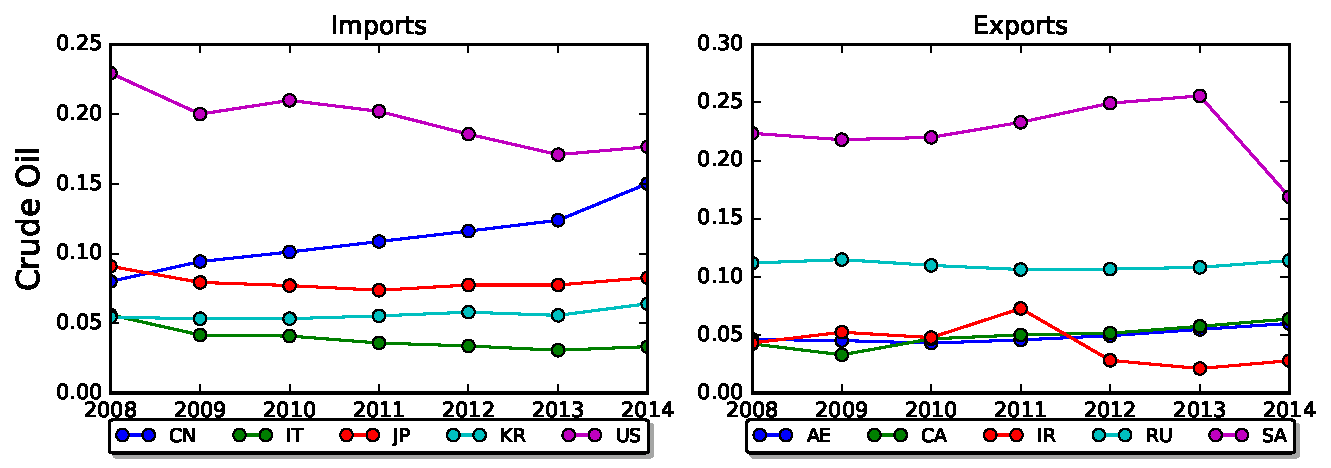
\includegraphics[scale=0.59]{plots/270900.pdf} \\
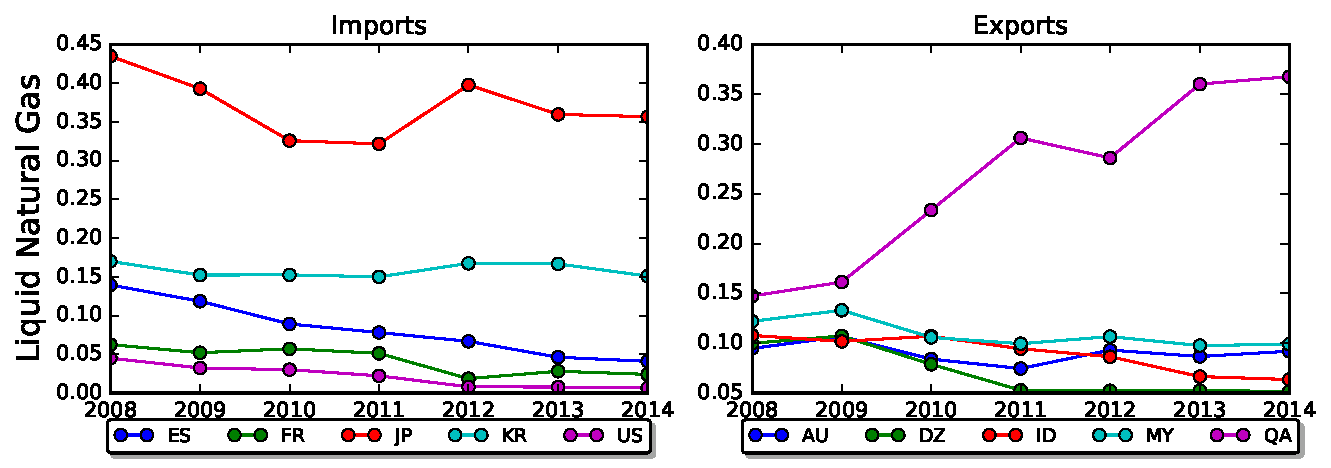
\includegraphics[scale=0.59]{plots/271111.pdf} \\
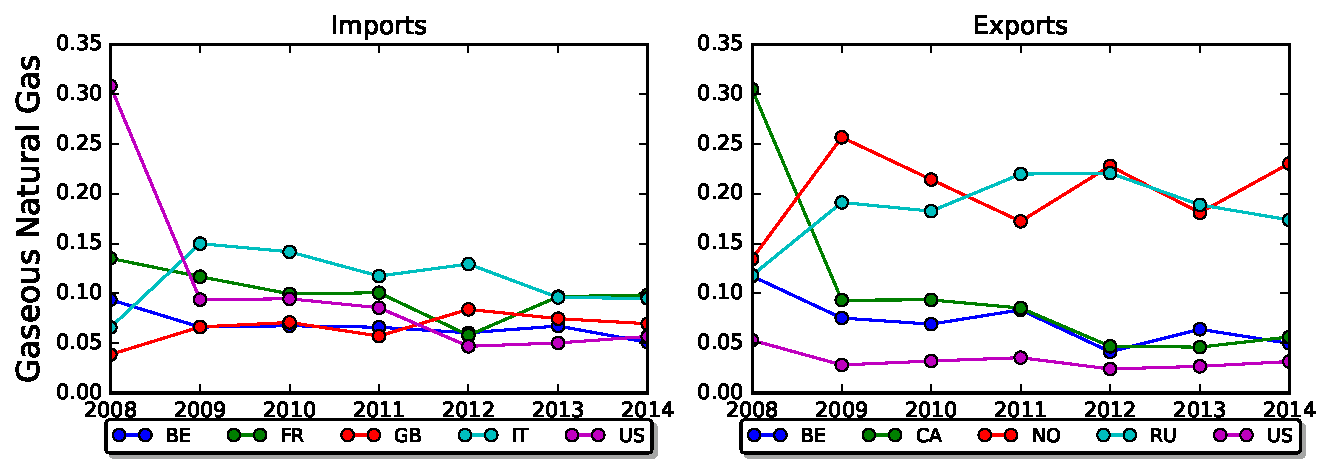
\includegraphics[scale=0.59]{plots/271121.pdf} \\ \par
} 
\footnotesize{Source: CEPII BACI; own calculations. \\
Countries: AE: United Arab Emirates; AU: Australia; BE: Belgium; CA: Canada; CN: China; DZ: Algeria; ES: Spain; FR: France; IR: Iran; IT: Italy; JP: Japan; KR: Korea; MY: Malaysia; NO: Norway; QA: Qatar; RU: Russia; SA: Saudi Arabia; US: United States.\\ 
Notes: The U.S. share of imports of all three products have decreased since 2008. China claims roughly 15 percent of crude oil imports in 2014, nearly doubling its share over seven year the period. Japan, traditionally the main player in LNG imports, had been closing LNG power plants until the nuclear disaster in 2011. Countries in Western Europe have generally decreased their reliance on LNG imports of all types and increased the use of renewable energy. Qatar has become increasingly dominant in the global trade of liquid natural gas. Trade between the U.S. and and Canada in gaseous-state natural gas fell sharply in 2009 in response to economic conditions and the shift towards horizontal wells. }
\end{figure}


\newpage 
 
\noindent \begin{figure} \label{fig:map}
  \caption{Changes to eigenvector centrality scores}
  {\centering
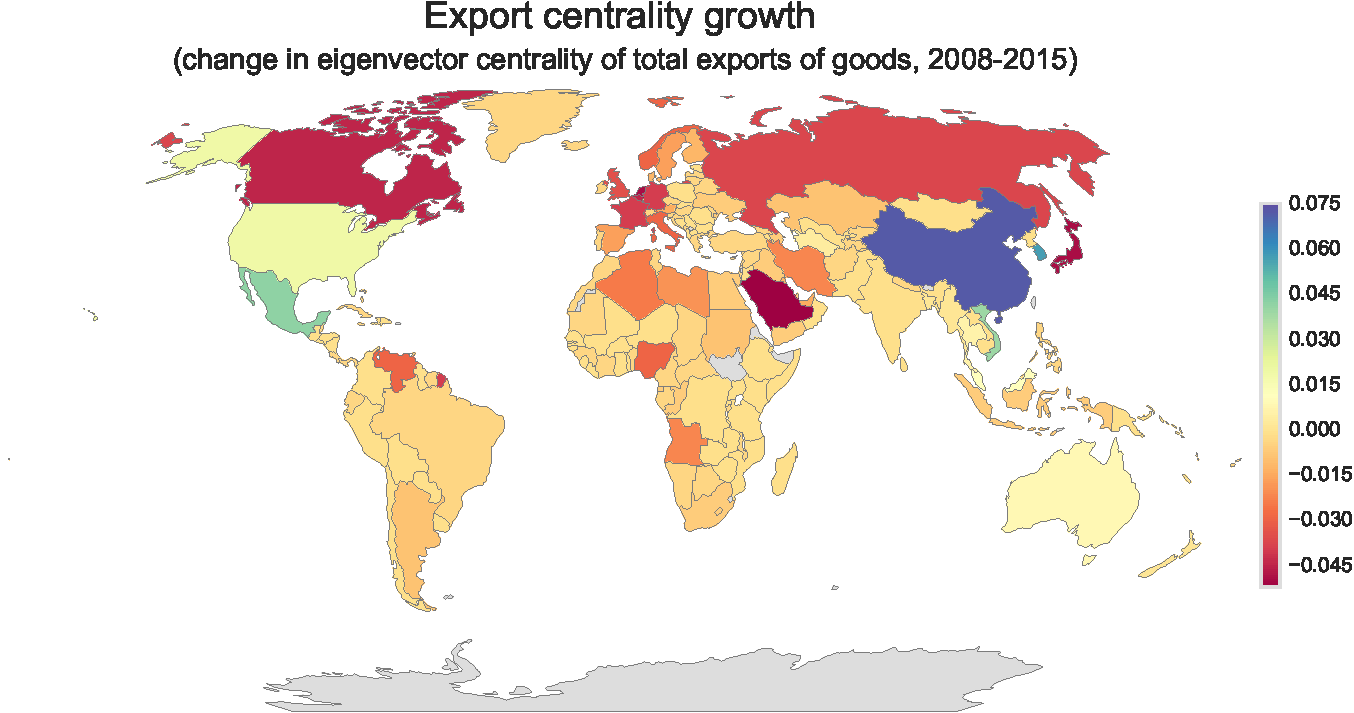
\includegraphics[scale=0.6]{map/exports_centrality_growth.pdf} \\
\vspace{3mm}

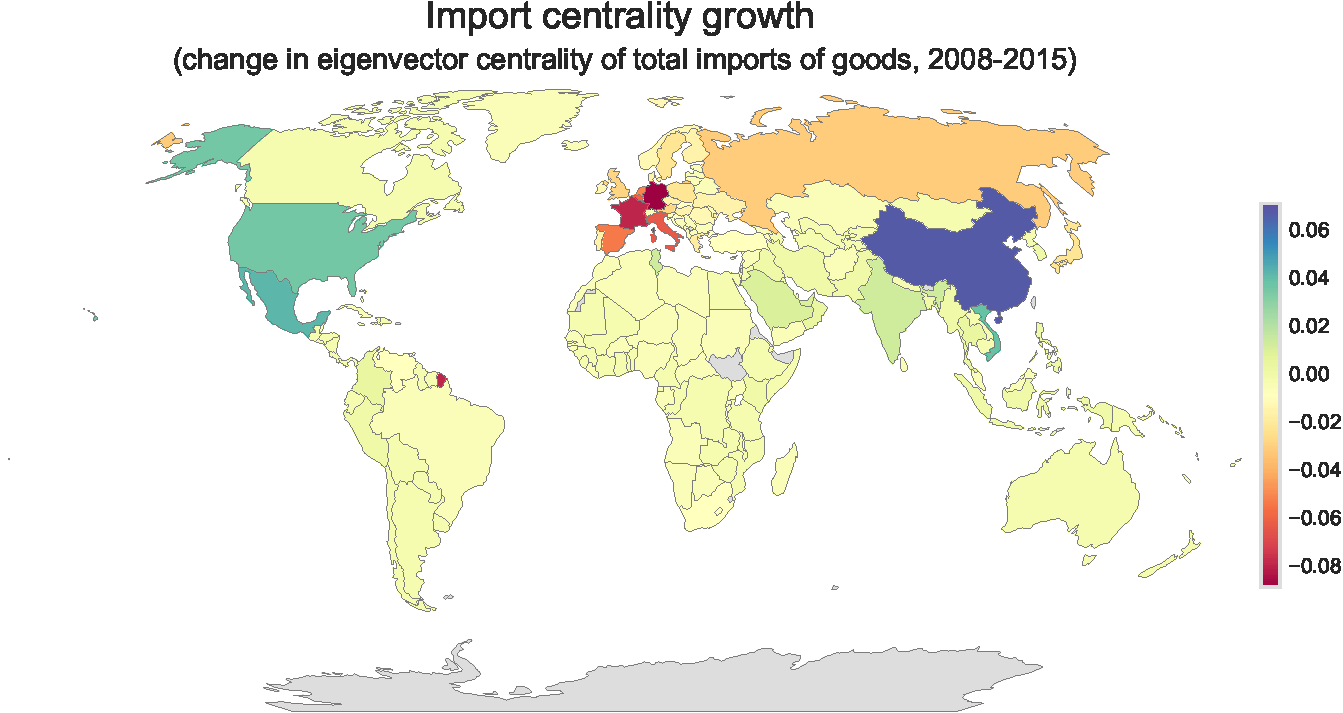
\includegraphics[scale=0.6]{map/imports_centrality_growth.pdf} \\ \par
} 
\footnotesize{Source: IMF Direction of Trade Statistics; own calculations. \\
Notes: Export growth has been very uneven since 2008, with exporters of primary commodities hit particularly hard. Saudi Arabia, Canada, Russia, Nigeria, and Venezuela are oil exporters who see their centrality in global exports fall by 2.5 points or more. Japan, much of the core eurozone, and the U.K. see export centrality reduced by three points or more. China improves its export centrality by 7.5 points in the eight year period. South Korea sees the second largest increase, followed by Mexico, Vietnam, the U.S., Malaysia, Australia, and Thailand. On the import side, China again grows by more than 7 points, followed by Hong Kong with an increase of 5.3 points. Mexico, Vietnam, and the U.S. all grow by more than 3 points, while India, Tunisia, Saudi Arabia, and the U.A.E. all grow by more than one point. The eurozone is the hardest hit. A long economic downturn has battered trade volumes, while trade partnerships between traditionally periphery countries strengthened.}
\end{figure}



\end{document}